\documentclass[12pt]{article}
\usepackage[utf8]{inputenc}

\usepackage{lmodern}

\usepackage{enumitem}
\usepackage[margin=2cm]{geometry}

\usepackage{amsmath, amsfonts, amssymb}
\usepackage{graphicx}
%\usepackage{subfigure}
\usepackage{tikz}
\usepackage{pgfplots}
\usepackage{multicol}

\usepackage{comment}
\usepackage{url}
\usepackage{calc}
\usepackage{subcaption}
\usepackage[indent=0pt]{parskip}
\usepackage{animate}

\usepackage{array}
\usepackage{blkarray,booktabs, bigstrut}
\usepackage{bigints}

\pgfplotsset{compat=1.16}

% MATH commands
\newcommand{\ga}{\left\langle}
\newcommand{\da}{\right\rangle}
\newcommand{\oa}{\left\lbrace}
\newcommand{\fa}{\right\rbrace}
\newcommand{\oc}{\left[}
\newcommand{\fc}{\right]}
\newcommand{\op}{\left(}
\newcommand{\fp}{\right)}

\newcommand{\bi}{\mathbf{i}}
\newcommand{\bj}{\mathbf{j}}
\newcommand{\bk}{\mathbf{k}}
\newcommand{\bF}{\mathbf{F}}

\newcommand{\mR}{\mathbb{R}}

\newcommand{\ra}{\rightarrow}
\newcommand{\Ra}{\Rightarrow}

\newcommand{\sech}{\mathrm{sech}\,}
\newcommand{\csch}{\mathrm{csch}\,}
\newcommand{\curl}{\mathrm{curl}\,}
\newcommand{\dive}{\mathrm{div}\,}

\newcommand{\ve}{\varepsilon}
\newcommand{\spc}{\vspace*{0.5cm}}

\DeclareMathOperator{\Ran}{Ran}
\DeclareMathOperator{\Dom}{Dom}

\newcommand{\exo}[1]{\noindent\textcolor{red}{\fbox{\textbf{Problem {#1}}}\hrulefill}\\\\ }
\newcommand{\qu}[4]{\noindent\textcolor{#4}{\fbox{\textbf{Section {#1} | Problem {#2}}} \hrulefill{{\fbox{\textbf{{#3} Points}}}}\\}}

\newcommand{\semester}{Fall 2023}

\newcommand{\CVup}{%
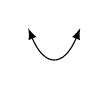
\begin{tikzpicture}
\draw[black, <->, >=latex] (-0.33, 0.5) .. controls (-0.125, 0) and (0.125, 0) .. (0.33, 0.5);
\end{tikzpicture}}

\newcommand{\CVupInc}{%
\begin{tikzpicture}
\draw[black, ->, >=latex] (0,0) .. controls (0.2, 0) and (0.4, 0.2) .. (0.5, 0.5);
\end{tikzpicture}}

\newcommand{\CVupDec}{%
\begin{tikzpicture}[rotate=270]
\draw[black, ->, >=latex] (0,0) .. controls (0.2, 0) and (0.4, 0.2) .. (0.5, 0.5);
\end{tikzpicture}}

\newcommand{\CVdown}{%
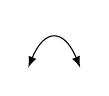
\begin{tikzpicture}
\draw[black, <->, >=latex] (-0.33, -0.5) .. controls (-0.125, 0) and (0.125, 0) .. (0.33, -0.5);
\end{tikzpicture}}

\newcommand{\CVdownInc}{%
\begin{tikzpicture}
\draw[black, ->, >=latex] (-0.5, -0.5) .. controls (-0.5, -0.3) and (-0.5, -0.1) .. (0,0);
\end{tikzpicture}}

\newcommand{\CVdownDec}{%
\begin{tikzpicture}[rotate=-90]
\draw[black, ->, >=latex] (-0.5, -0.5) .. controls (-0.5, -0.3) and (-0.5, -0.1) .. (0,0);
\end{tikzpicture}}

\begin{document}
	\noindent \hrulefill \\
	MATH-244 \semester \hfill Practice Problems Solutions\\
	Section 16.9 \hfill Pierre-Olivier Paris{\'e} \\\vspace*{-1cm}
	
	\noindent\hrulefill
	
	\spc	

	\exo{6}
	By the Divergence Theorem, we have
		\begin{align*}
		\iint_S \vec{F} \cdot d\vec{S} = \iiint_E \dive \vec{F} \, dV .
		\end{align*}
	
	The surface is a rectangular box $S$. The inside of the box is
		\begin{align*}
		E = \{ (x, y, z) \, : \, 0 \leq x \leq a , 0 \leq y \leq b , 0 \leq z \leq c \} .
		\end{align*}
	We have
		\begin{align*}
		\dive \vec{F} = 2xyz + 2xyz + 2xyz = 6xyz .
		\end{align*}
	So, we obtain
		\begin{align*}
		\iint_S \vec{F} \cdot d\vec{S} = \int_0^c \int_0^b \int_0^a 6xyz \, dxdydz = 3a^2 b^2 c^2/4 .
		\end{align*}
	
	\spc
	
	\exo{18}
	Let $S_1$ be the bottom of the paraboloid. This is the disk
		\begin{align*}
		S_1 = \{ (x, y, z) \, : \, x^2 + y^2 \leq 1 , \, z = 1 \} .
		\end{align*}
	Let $\tilde{S} := S \cup S_1$, with the outward orientation. By the Divergence Theorem, we have
		\begin{align*}
		\iint_{\tilde{S}} \vec{F} \cdot d\vec{S} = \iiint_E \dive \vec{F} \, dV .
		\end{align*}
	The solid $E$ bounded by $\tilde{S}$ is
		\begin{align*}
		E = \{ (x, y, z) \, : \, x^2 + y^2 \leq 1 , 1 \leq z \leq 2 - x^2 - y^2 \} .
		\end{align*}
	The divergence of $\vec{F}$ is
		\begin{align*}
		\dive \vec{F} = 0 + 0 + 1 = 1 .
		\end{align*}
	So, we obtain
		\begin{align*}
		\iint_{\tilde{S}} \vec{F} \cdot d\vec{S} = \iint_{D} \Big( \int_1^{2 - x^2 - y^2} 1 \, dz \, \Big) dA = \iint_D 1 - x^2 - y^2 \, dA ,
		\end{align*}
	where $D := \{  (x, y) \, : \, x^2 + y^2 \leq 1 \}$. We can compute this integral by passing to polar coordinates. We then obtain
		\begin{align*}
		\int_0^{2\pi} \int_0^1 (1 - r^2) r \, dr d\theta = \pi/2 .
		\end{align*}
	The flux of $\vec{F}$ through $\tilde{S}$ is then $\pi/2$.
	
	This is not exactly the flux of $\vec{F}$ through $S$. To obtain the flux through $S$, we have to write
		\begin{align*}
		\pi/2 = \iint_{\tilde{S}} \vec{F} \cdot d\vec{S} = \iint_S \vec{F} \cdot d\vec{S} + \iint_{S_1} \vec{F} \cdot d\vec{S} 
		\end{align*}
	and so
		\begin{align*}
		\iint_S \vec{F} \cdot d \vec{S} = \pi/2 - \iint_{S_1} \vec{F} \cdot d\vec{S} .
		\end{align*}
	Recall that $\tilde{S}$ had the outward orientation, so to be consistent with that choice, $S_1$ has the downward orientation. A normal vector to $S_1$ pointing downward is $\vec{n} = \left\langle 0, 0, -1 \right\rangle$ and so
		\begin{align*}
		\iint_{S_1} \vec{F} \cdot d\vec{S} = \iint_{S_1} \vec{F} \cdot \left\langle 0, 0, -1 \right\rangle \, dS = \iint_{S_1} -z \, dS = - \iint_{S_1} z \, dS
		\end{align*}
	But, when on $S_1$, we have $z = 1$, and so the double integral represents the area of the disk. The disk has radius $1$ and we then obtain
		\begin{align*}
		\iint_S \vec{F} \cdot d \vec{S} = \pi/2 + \pi = 3\pi/2 .
		\end{align*}


\end{document}